% Options for packages loaded elsewhere
\PassOptionsToPackage{unicode}{hyperref}
\PassOptionsToPackage{hyphens}{url}
%
\documentclass[
]{article}
\usepackage{amsmath,amssymb}
\usepackage{lmodern}
\usepackage{iftex}
\ifPDFTeX
  \usepackage[T1]{fontenc}
  \usepackage[utf8]{inputenc}
  \usepackage{textcomp} % provide euro and other symbols
\else % if luatex or xetex
  \usepackage{unicode-math}
  \defaultfontfeatures{Scale=MatchLowercase}
  \defaultfontfeatures[\rmfamily]{Ligatures=TeX,Scale=1}
\fi
% Use upquote if available, for straight quotes in verbatim environments
\IfFileExists{upquote.sty}{\usepackage{upquote}}{}
\IfFileExists{microtype.sty}{% use microtype if available
  \usepackage[]{microtype}
  \UseMicrotypeSet[protrusion]{basicmath} % disable protrusion for tt fonts
}{}
\makeatletter
\@ifundefined{KOMAClassName}{% if non-KOMA class
  \IfFileExists{parskip.sty}{%
    \usepackage{parskip}
  }{% else
    \setlength{\parindent}{0pt}
    \setlength{\parskip}{6pt plus 2pt minus 1pt}}
}{% if KOMA class
  \KOMAoptions{parskip=half}}
\makeatother
\usepackage{xcolor}
\IfFileExists{xurl.sty}{\usepackage{xurl}}{} % add URL line breaks if available
\IfFileExists{bookmark.sty}{\usepackage{bookmark}}{\usepackage{hyperref}}
\hypersetup{
  pdftitle={Baseball Hall of Fame Report},
  pdfauthor={Andy, Dante, Kai, and Kobe},
  hidelinks,
  pdfcreator={LaTeX via pandoc}}
\urlstyle{same} % disable monospaced font for URLs
\usepackage[margin=1in]{geometry}
\usepackage{graphicx}
\makeatletter
\def\maxwidth{\ifdim\Gin@nat@width>\linewidth\linewidth\else\Gin@nat@width\fi}
\def\maxheight{\ifdim\Gin@nat@height>\textheight\textheight\else\Gin@nat@height\fi}
\makeatother
% Scale images if necessary, so that they will not overflow the page
% margins by default, and it is still possible to overwrite the defaults
% using explicit options in \includegraphics[width, height, ...]{}
\setkeys{Gin}{width=\maxwidth,height=\maxheight,keepaspectratio}
% Set default figure placement to htbp
\makeatletter
\def\fps@figure{htbp}
\makeatother
\setlength{\emergencystretch}{3em} % prevent overfull lines
\providecommand{\tightlist}{%
  \setlength{\itemsep}{0pt}\setlength{\parskip}{0pt}}
\setcounter{secnumdepth}{-\maxdimen} % remove section numbering
\usepackage{float}
\floatplacement{figure}{H}
\floatplacement{table}{H}
\ifLuaTeX
  \usepackage{selnolig}  % disable illegal ligatures
\fi

\title{Baseball Hall of Fame Report}
\author{Andy, Dante, Kai, and Kobe}
\date{2023-03-14}

\begin{document}
\maketitle

\fontsize{9}{13}
\selectfont

\hypertarget{introduction}{%
\section{Introduction}\label{introduction}}

\hypertarget{background-and-motivation}{%
\subsection{Background and Motivation}\label{background-and-motivation}}

The data we are working with is career baseball statistics. The data was
collected from official scorekeepers who went to every Major League
Baseball game and tracked various outcomes players had over the course
of each game. For our finished data set, those statistics were added up
at the end of each baseball season and also at the end of each player's
career. The motivation for the scorekeepers to track the data was that
they were paid, either by the home team, the league as a whole, or the
local newspaper to track these statistics to keep baseball fans
informed.

One motivation for our research question was to better understand which
variables are associated with a successful hall of fame induction.
Another motivation for our research is an extension of the first, which
is for us to predict which players will be inducted into the hall of
fame in the future.

\hypertarget{research-question}{%
\subsection{Research Question}\label{research-question}}

As such, our first research question is what factors are associated with
a position player being inducted into the hall of fame and whether we
can create a model that uses these factors to predict what players will
make the hall of fame. Our other research question is what factors are a
associated with whether a pitcher is inducted into the hall of fame and
whether we can create a model that uses these factors to predict what
pitchers will make the hall of fame.

We'll be using R version \texttt{2022.02.3+492} throughout this project,
so please update to at least R version \texttt{2022.02.3+492} to be able
to replicate our process.

\hypertarget{data-description}{%
\section{Data Description}\label{data-description}}

Our data consist of mostly quantitative variables mixed in with some
categorical variables. Most baseball metrics come in quantitative form
so it is often hard to obtain categorical measurements unless they come
directly from the quantitative variables themselves. However, some
categorical variables we may use include factors such as year, league,
team, and possibly some other categorical variables that are computed
from other quantitative variables. One other potential categorical
variable would be a binary variable indicating whether a player was
publicly suspected to use steroids or not according to ESPN, MLB PED
test results, and miscellaneous PED related court documents.

Furthermore, we are splitting this project into two parts: batters and
pitchers. Thus, there is a need to split the data; in other words, we
will have two different data sets, since metrics for batters and
pitchers are vastly different. However, we will still be predicting the
same variable: hall of fame. Hall of fame is a binary categorical
variable, indicating whether a player was inducted into the hall of fame
or not. In addition, we made sure to only include players who were on a
hall of fame ballot at some point. In total, we have around 750
observations in the position players data set and 400 observations in
the pitching data set.

\hypertarget{exploratory-data-analysis}{%
\section{Exploratory Data Analysis}\label{exploratory-data-analysis}}

\hypertarget{correlation-plots}{%
\subsection{Correlation Plots}\label{correlation-plots}}

\begin{figure}

{\centering 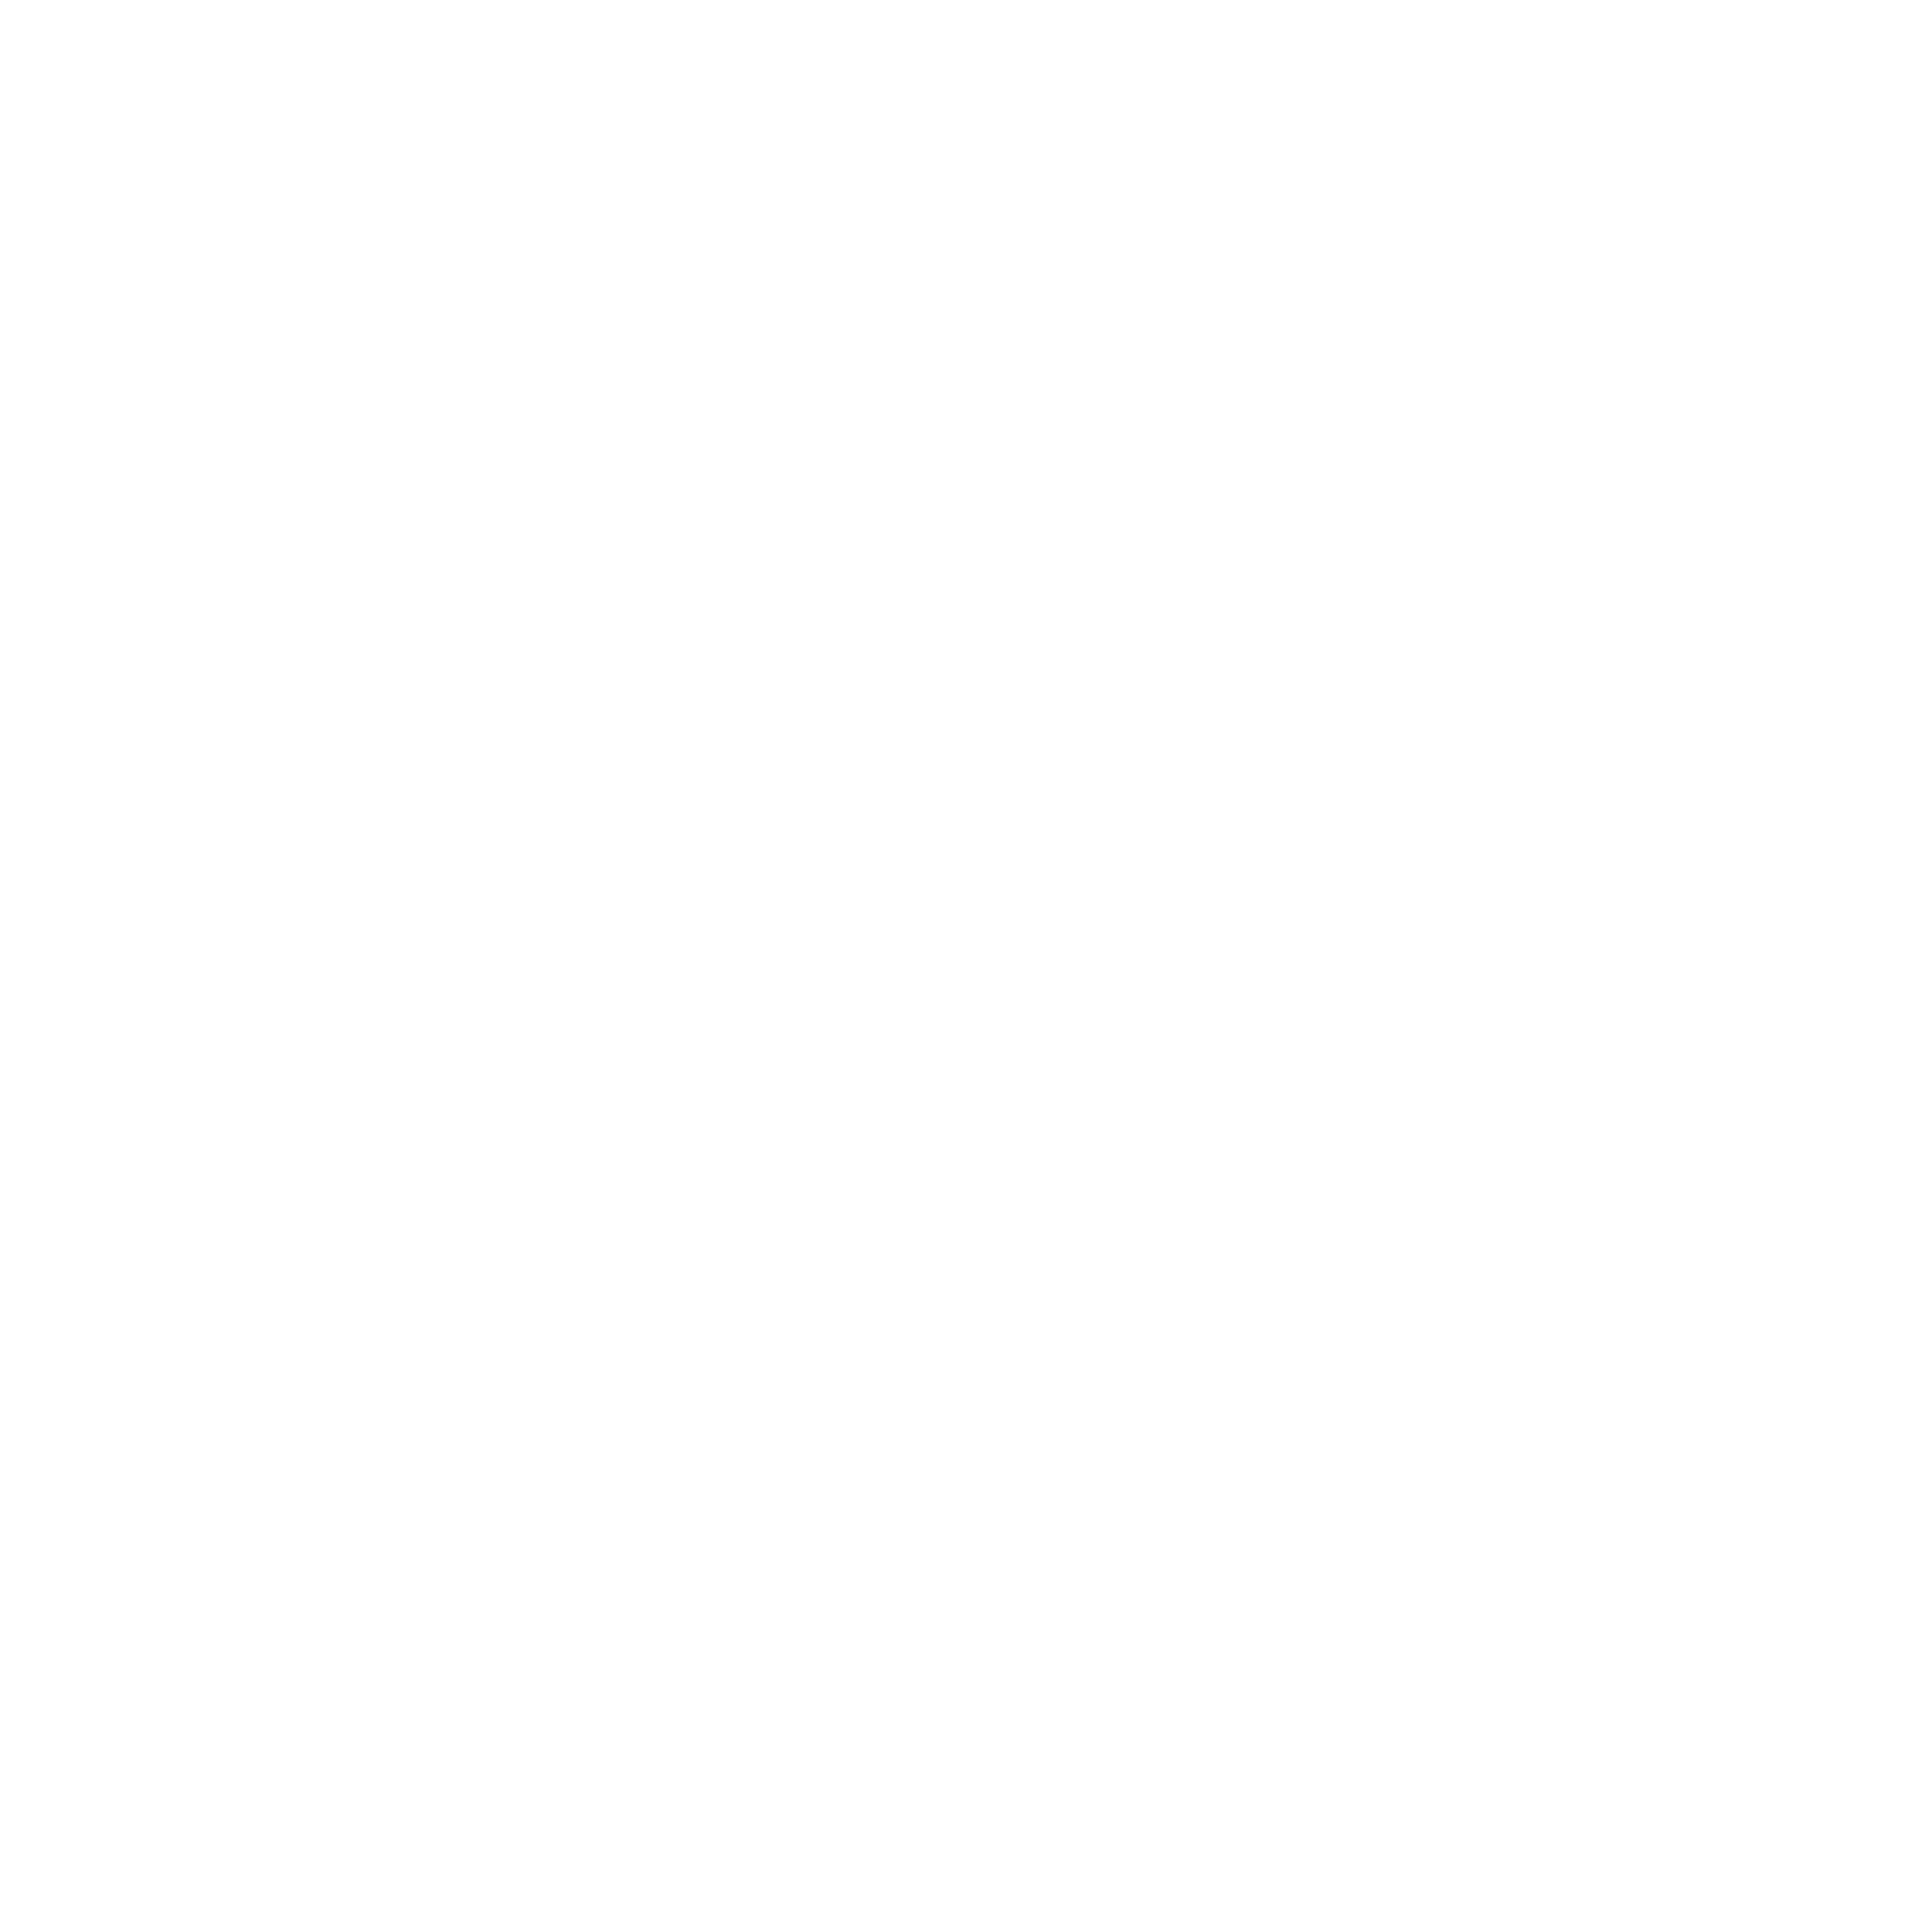
\includegraphics[width=0.49\linewidth,height=0.2\textheight]{../corr_pos} 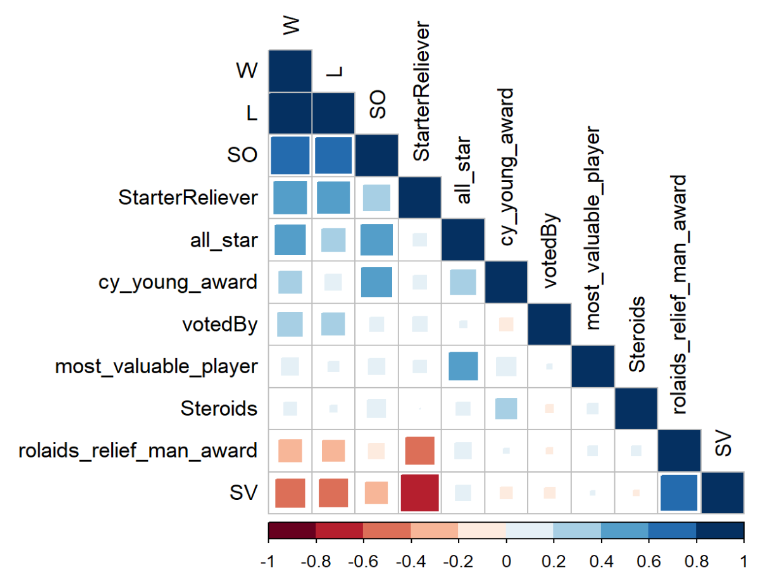
\includegraphics[width=0.49\linewidth,height=0.2\textheight]{../Plots/corr_pitch} 

}

\caption{Correlation Plots}\label{fig:unnamed-chunk-1}
\end{figure}

We can see that a few of our variables have multicollinearity,
especially the hitting rate stats which are amalgamations of counting
hit stats. However not all predictors are as highly correlated with each
other. So, we will carry on with our analysis using most of the
variables, since we deem those variables as important factors.

\hypertarget{awards-eda-steroids-svd-plots}{%
\subsection{Awards EDA \& Steroids SVD
plots}\label{awards-eda-steroids-svd-plots}}

\begin{figure}

{\centering 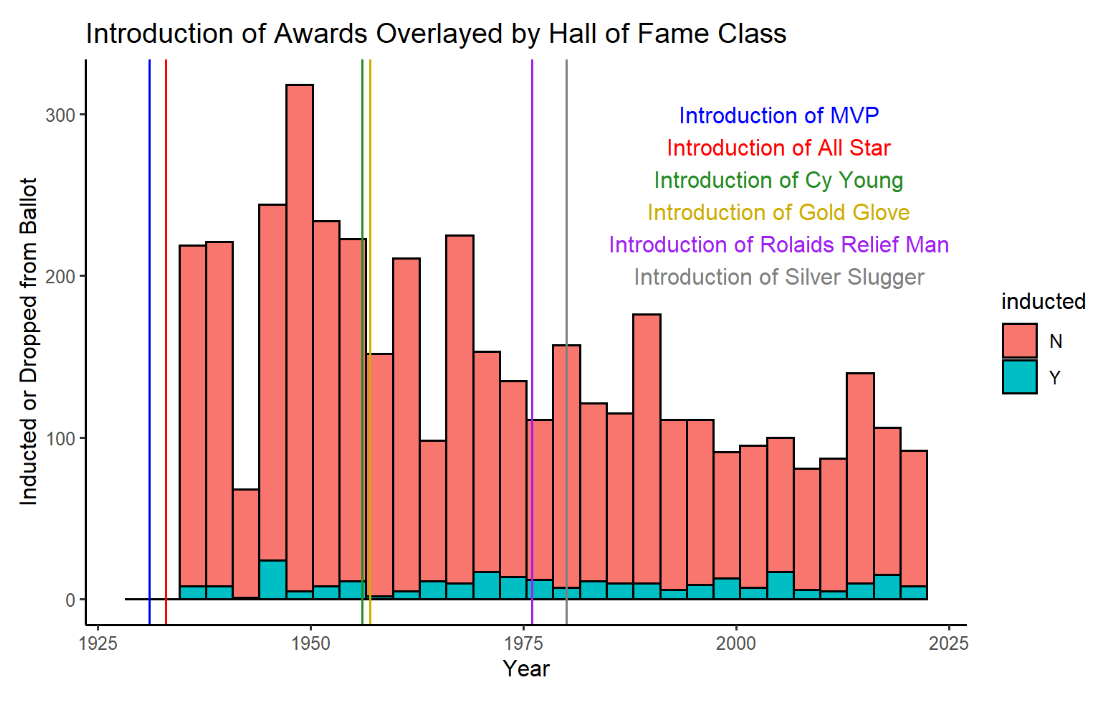
\includegraphics[width=0.49\linewidth,height=0.2\textheight]{../Plots/award_eda} 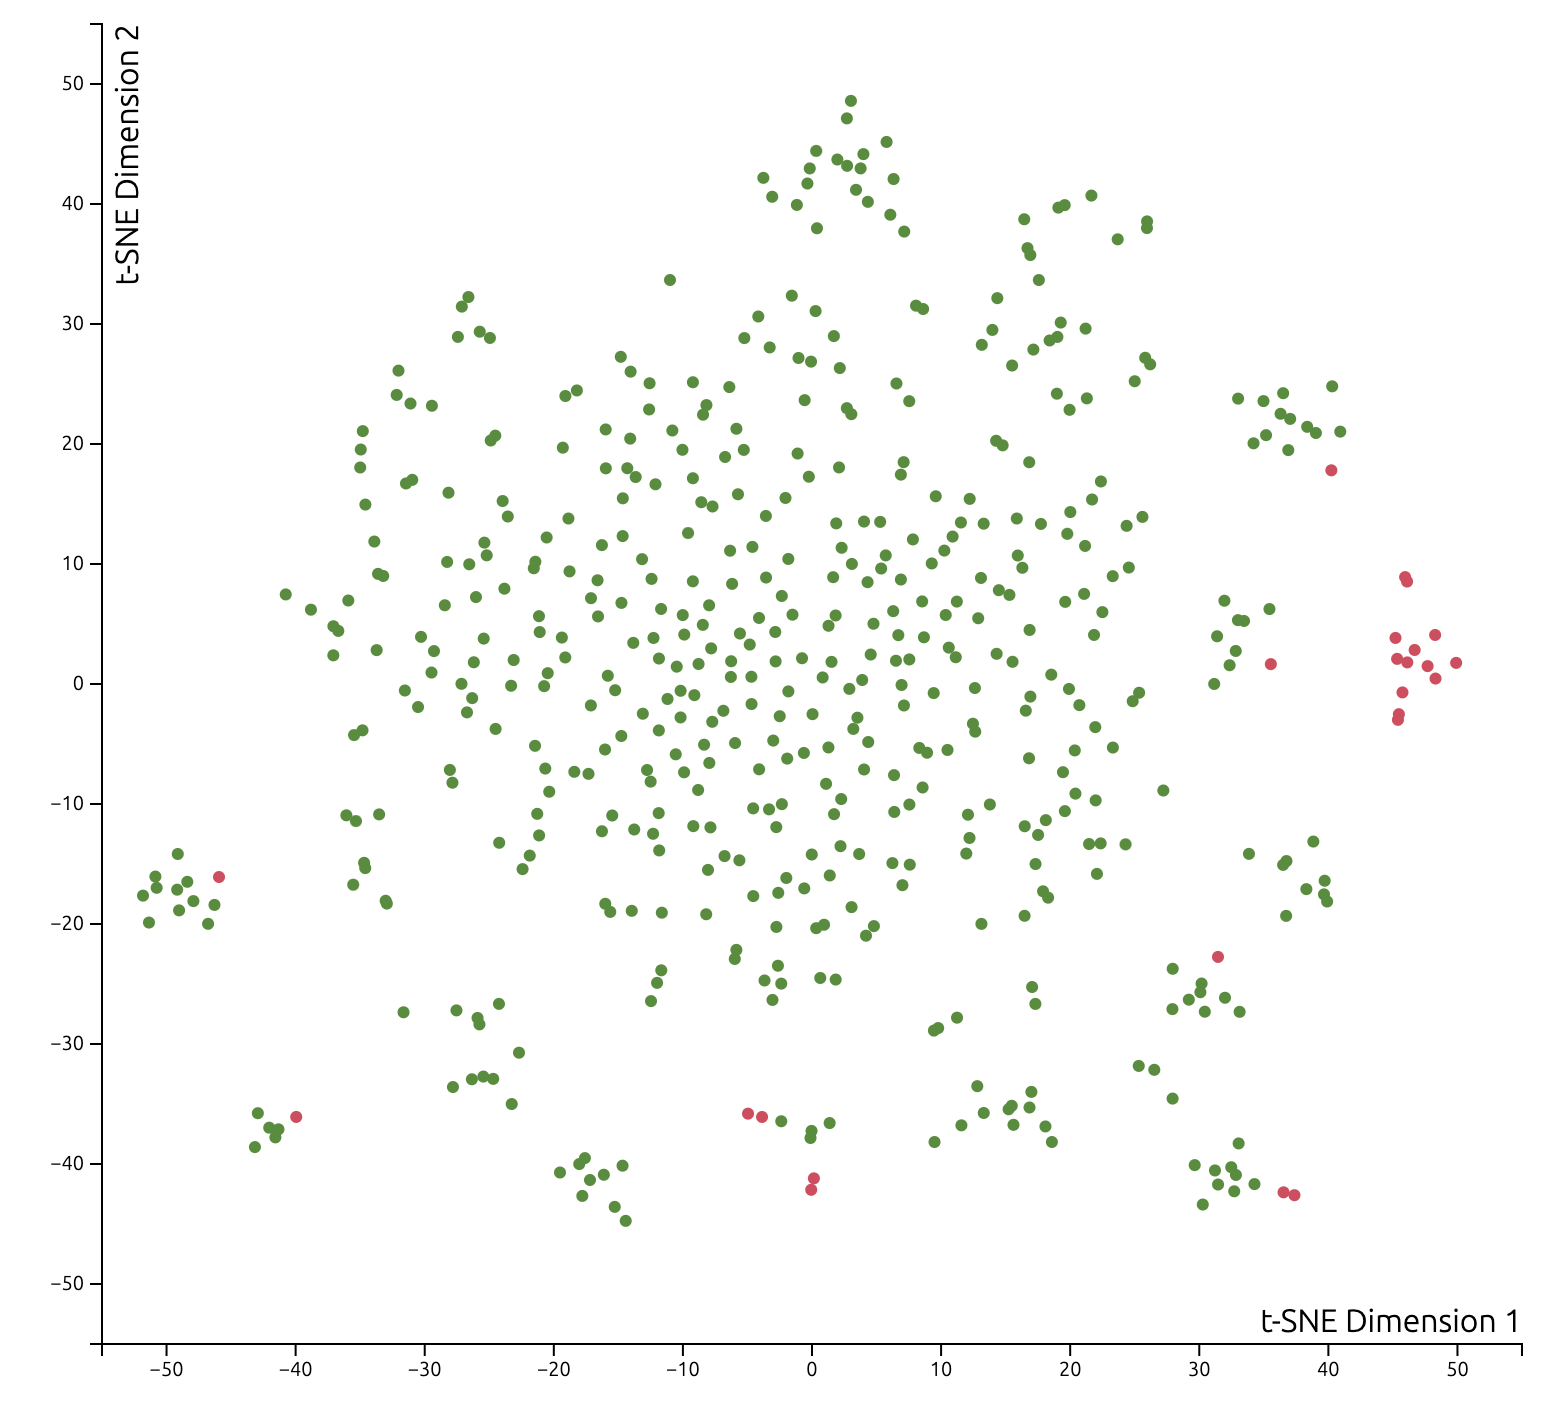
\includegraphics[width=0.49\linewidth,height=0.2\textheight]{../Plots/steroids} 

}

\caption{Awards and Election Proportion, tSNE Plot}\label{fig:unnamed-chunk-2}
\end{figure}

A time plot showing the total counts of players inducted and players no
longer eligible for the normal ballot. Introduction of awards overlaid
to explain a lack of significance which we might see for accolades
introduced in the mid 20th century after a large proportion of total
players who have ever been on ballot had already been inducted or
dropped off of the ballot. A player gets dropped off the ballot when
they have been on the ballot for more than 10 years or received 5\% or
less of the votes by all voters. Additionally, a voter can only vote for
up to 10 players on any specific ballot. Below are the cumulative
percentages of the proportion of players who had either been inducted
into the hall of fame or dropped off the ballot by the time each award
was introduced. As we see, almost 2/3 of players who had ever been on
the ballot had their Hall of Fame candidacy decided before the
introduction of the Silver Slugger award.

\begin{itemize}
\tightlist
\item
  Before MVP \& All-Star -- 0\%
\item
  Before Cy Young and Gold Glove Award \textasciitilde{} 33.9\%
\item
  Before Rolaids Reliever of the Year and Silver Slugger Award
  \textasciitilde{} 61\%
\end{itemize}

Using t-SNE, a dimension reduction approach, we can visualize the many
variables we have into two principal components, which is what is seen
here. As we can tell from this clustering, many of the position players
who took steroids throughout their career colored in
\(\textcolor{red}{red}\) have eerily similar career statistics. As such,
it made sense to make \texttt{Steroids} its own variable. The axes have
no reasonable interpretation as is with some dimension reduction
techniques.

\hypertarget{methods}{%
\section{Methods}\label{methods}}

\hypertarget{family-wise-error}{%
\subsection{Family-wise Error}\label{family-wise-error}}

For our hypothesis testing, since we use so many predictors for both
models, our family wise error rate would be higher than our intended
level. As such, we are going to use the Bonferonni correction. This
gives us that the significant threshold for p-values are 0.0015 for
Position Players and 0.0042 for Pitchers.

\hypertarget{assumptions}{%
\subsection{Assumptions}\label{assumptions}}

We are assuming a constant probability of being elected into the Hall of
Fame throughout the history of baseball, a necessary assumption for
logistic regression with a binomial random variable response. This seems
reasonable according to our \texttt{Awards\ EDA}. Additionally, we are
assuming homoscedasticity and normally distributed errors which we will
show through \texttt{qqplots} after we have filtered our data properly.
Lastly, we are assuming each observation is independent of one another,
which we must be careful with. Baseball is a series of one-on-one match
ups between a batter and a pitcher. It is zero-sum, meaning the success
of a pitcher is correlated to the failure of a batter. However, because
the number of times any hitter will face the same pitcher is negligible
compared to the amount of pitchers the batter will otherwise face
throughout their entire career, we will assume independence.

\hypertarget{data-wrangling}{%
\subsection{Data Wrangling}\label{data-wrangling}}

\begin{itemize}
\item
  For batters, we summed across playerID groups in the ``Batting'' data
  frame in the Lahman package. This allowed us to see career totals for
  rate and counting stats for each observation (player) like batting
  average (AVG), walks (BB), and total hits for each of the four base
  categories (1B, 2B, 3B, HR). We joined a pivoted ``award'' data frame
  that added approximately 20 accolade predictors for each observation.
  This includes total all-star selections, Most Valuable Player awards
  won, Silver Sluggers, etc.
\item
  For pitcher, we sumed across playerID groups in the ``Pitching'' data
  frame in the Lahman package. This allowed us to see career totals for
  recognizable rate and counting stats for each observation (pitcher)
  like innings pitched (IP), strike outs (SO), earned runs (ER), and we
  additionally mutated
  \(\frac{9 \times \text{Earned Runs}}{\text{Innings Pitched}}\) and
  \(\frac{\text{Walks} + \text{Hits}}{\text{Innings Pitched}}\) to get
  the all important ERA (Earned Run Average) and WHIP (Walks plus Hits
  per Inning Pitched) rates. We then joined a pivoted ``award'' data
  frame that added approximately 20 accolade predictors for each
  observation, this includes total all-star selections, Cy Young awards
  won, Gold Gloves, etc.
\end{itemize}

The initial AIC's (approximately 220 and 80 for our Position Player and
Pitcher models respectively) from our step() selection process and some
rather large Cook's Distance values indicated the necessity to mutate
additional predictors. Players like Barry Bonds, Roger Clemens, and
Manny Ramirez were being flagged by our Cook's Distance Plots as
uncharacteristically not elected into the Hall of Fame.

\begin{itemize}
\item
  The late 90's, early 2000's Steroids era of baseball altered the way
  the Baseball Writers Association of America (BBWAA) voters viewed the
  careers of some players in spite of otherwise Hall of Fame worthy
  numbers. And so, using web scraped data from ESPN and Bay Area
  Laboratory Co-operative (BALCO) court documents, we mutated a binary
  0/1 column that indicated if a player was indicted on any sort of
  performance enhancing drug (PED) scandal.
\item
  We then ran our step() model selection process again, and while we
  obtained better AIC values, we felt we could do better. We understood
  what the baseball writers considered important to be elected into the
  Hall of Fame was period and cohort dependent. Therefore, we mutated a
  column that signified which of two committees elected a player into
  the Hall of Fame; BBWAA or the Veterans Committee. The BBWAA typically
  votes players 5-15 years after their retirement, while the Veterans
  Committee typically votes players based on high batting averages or
  nepotism from the dead-ball era of baseball (1880-1920).
\item
  For position players specifically, we felt the need to add a variable
  which identifies the primary position of a player throughout their
  career. This is important because of something called ``Positional
  Adjustment''. Based on the defensive difficulty of each position, a
  player is typically expected to perform at a certain offensive level
  to be considered above replacement level. For example, a first-baseman
  who has what is considered an easy position defensively, is expected
  to perform far better offensively than a player at the catcher
  position, which is considered the most difficult defensive position
  according to FanGraphs Positional Adjustment.
\item
  For pitchers, preliminary variable selection via the step() function
  revealed the importance of relief pitcher accolades. Relief pitchers
  are a subset of pitchers who typically pitch \textasciitilde{} 60
  innings a season. We felt the need for our model to be differentiate
  between a starter and relief pitcher, and so we mutated such a
  predictor. This variable was accurate at identification with a cutoff
  of 60 innings per season after cross-referencing with 20 starters and
  20 relievers.
\end{itemize}

\hypertarget{model-selection}{%
\subsection{Model Selection}\label{model-selection}}

For our model building, we used essentially every possible variable that
could potentially be useful and did not contain more than 30 missing
observations. As such, we started our process with even larger models
than ones we already had To narrow down the number of covariates, we
used step-wise model selection that goes both forwards and backwards,
allowing us to test a large number of models. Since we are more focused
on the prediction aspect, as we wanted to be able to predict current
eligible players, we chose to use AIC as our primary criteria for model
selection over other criteria such as BIC.

\hypertarget{results}{%
\section{Results}\label{results}}

These tables are the summary information of the models we obtained from
many iterations of trying different variables for both pitchers and
position players. Further, the first iteration is considered the
``base'' model which includes all the basic measurements in our dataset
as it doesn't include manipulated data like \texttt{steroids} and
\texttt{votedBy}, both variables which needed further research to
obtain. The second iteration includes the variables we didn't include in
the first iteration whilst the third and final model includes
interactions of any variables as well. Thus, the third iteration can be
considered the most complex model out of the 3.

One thing that is important to note is how, for both models, the number
of observations gets higher with once we arrive at the final model. This
is due to some of the variables having missing values in them, so once
we eliminated that variable, it allowed us to add those observations
back into the model. As a result, our final models use more observations
compared to the previous models.

As you can observe, the AIC for the models go down as we clean up the
variables and add interactions, so we ended up settling with the last
model which gave us the lowest AIC.

\begin{table}[H] \centering 
  \caption{Pitchers Model(s)} 
  \label{} 
\tiny 
\begin{tabular}{@{\extracolsep{5pt}}lccc} 
\\[-1.8ex]\hline 
\hline \\[-1.8ex] 
 & \multicolumn{3}{c}{\textit{Dependent variable:}} \\ 
\cline{2-4} 
\\[-1.8ex] & \multicolumn{3}{c}{wein} \\ 
 & Iteration 1 & Iteration 2 & Iteration 3 \\ 
\\[-1.8ex] & (1) & (2) & (3)\\ 
\hline \\[-1.8ex] 
 W & 0.054$^{***}$ (0.010) & 0.076$^{***}$ (0.016) & 0.085$^{***}$ (0.023) \\ 
  ERA & $-$2.048$^{*}$ (1.107) & $-$3.089$^{**}$ (1.393) &  \\ 
  all\_star & 0.479$^{***}$ (0.134) & 0.488$^{***}$ (0.154) & 1.048$^{***}$ (0.275) \\ 
  WHIP & $-$4.454 (5.471) & 1.672 (6.571) &  \\ 
  SO & $-$0.0002 (0.001) & 0.00004 (0.001) & 0.001 (0.001) \\ 
  gold\_glove & 0.163 (0.244) & 0.093 (0.338) &  \\ 
  SV & 0.012$^{***}$ (0.004) & 0.022$^{***}$ (0.007) &  \\ 
  cy\_young\_award & $-$1.025$^{**}$ (0.500) & 0.939 (0.797) & 1.938$^{*}$ (1.087) \\ 
  votedByVeterans &  &  & 9.495$^{***}$ (2.313) \\ 
  StarterRelieverStarter &  &  & $-$7.384$^{*}$ (3.983) \\ 
  SV:StarterRelieverReliever &  &  & 0.014 (0.010) \\ 
  SV:StarterRelieverStarter &  &  & 0.100$^{**}$ (0.043) \\ 
  StarterRelieverReliever:rolaids\_relief\_man\_award &  &  & 1.439 (0.972) \\ 
  StarterRelieverStarter:rolaids\_relief\_man\_award &  &  & $-$0.234 (2,240.016) \\ 
  Steroids:most\_valuable\_player &  &  & $-$37.590 (11,865.490) \\ 
  Steroids &  & $-$38.847 (2,007.568) & $-$15.584 (5,014.066) \\ 
  most\_valuable\_player & 0.291 (1.072) & 0.876 (1.281) & 3.915$^{**}$ (1.914) \\ 
  pitching\_triple\_crown & 1.294$^{*}$ (0.751) & 1.168 (0.887) &  \\ 
  rolaids\_relief\_man\_award & 1.060$^{**}$ (0.417) & 1.078$^{*}$ (0.559) &  \\ 
  nice\_guy\_awards & $-$0.632 (0.476) & $-$1.427$^{**}$ (0.677) &  \\ 
  Constant & $-$2.057 (4.858) & $-$11.977$^{*}$ (6.405) & $-$22.946$^{***}$ (5.898) \\ 
 \hline \\[-1.8ex] 
Observations & 342 & 342 & 401 \\ 
Log Likelihood & $-$46.083 & $-$33.545 & $-$19.255 \\ 
Akaike Inf. Crit. & 118.167 & 95.090 & 66.511 \\ 
\hline 
\hline \\[-1.8ex] 
\textit{Note:}  & \multicolumn{3}{r}{$^{*}$p$<$0.1; $^{**}$p$<$0.05; $^{***}$p$<$0.01} \\ 
\end{tabular} 
\end{table}

\begin{table}[H] \centering 
  \caption{Position Players Model(s)} 
  \label{} 
\tiny 
\begin{tabular}{@{\extracolsep{5pt}}lccc} 
\\[-1.8ex]\hline 
\hline \\[-1.8ex] 
 & \multicolumn{3}{c}{\textit{Dependent variable:}} \\ 
\cline{2-4} 
\\[-1.8ex] & \multicolumn{3}{c}{wein} \\ 
 & Iteration 1 & Iteration 2 & Iteration 3 \\ 
\\[-1.8ex] & (1) & (2) & (3)\\ 
\hline \\[-1.8ex] 
 G & 0.004 (0.003) & 0.004 (0.003) &  \\ 
  AB & 0.004 (0.003) & 0.003 (0.003) &  \\ 
  R & 0.009$^{**}$ (0.004) & 0.011$^{***}$ (0.004) & 0.011$^{**}$ (0.005) \\ 
  H & $-$0.019$^{**}$ (0.009) & $-$0.019$^{**}$ (0.010) &  \\ 
  HR & $-$0.010 (0.007) & $-$0.008 (0.007) & 0.031$^{**}$ (0.015) \\ 
  RBI & 0.002 (0.002) & 0.003 (0.003) & 0.008 (0.006) \\ 
  SB & $-$0.003 (0.002) & $-$0.003 (0.002) & 0.011$^{*}$ (0.007) \\ 
  BB & 0.004 (0.004) & 0.002 (0.004) &  \\ 
  PrimaryLgNL & $-$0.206 (0.466) & $-$0.269 (0.479) &  \\ 
  Pos2B:HR &  &  & $-$0.064$^{***}$ (0.024) \\ 
  Pos3B:HR &  &  & $-$0.022 (0.024) \\ 
  PosC:HR &  &  & $-$0.025 (0.026) \\ 
  PosCF:HR &  &  & $-$0.033 (0.082) \\ 
  PosDH:HR &  &  & 0.021 (0.051) \\ 
  PosLF:HR &  &  & $-$0.001 (0.017) \\ 
  PosRF:HR &  &  & $-$0.048$^{**}$ (0.023) \\ 
  PosSS:HR &  &  & $-$0.079$^{**}$ (0.031) \\ 
  all\_star:most\_valuable\_player &  &  & $-$0.295 (0.261) \\ 
  Steroids:SLG &  &  & $-$105.800 (97.506) \\ 
  all\_star & 0.494$^{***}$ (0.089) & 0.530$^{***}$ (0.097) & 1.321$^{***}$ (0.387) \\ 
  most\_valuable\_player & 0.373 (0.451) & 0.200 (0.486) & 4.087$^{*}$ (2.150) \\ 
  AVG & 214.493$^{***}$ (78.055) & 212.914$^{***}$ (80.415) & 140.045$^{**}$ (55.842) \\ 
  OBP & $-$56.691 (45.829) & $-$45.906 (47.227) &  \\ 
  SLG & 8.154 (19.633) & $-$0.116 (20.421) &  \\ 
  Steroids &  & $-$3.836$^{**}$ (1.663) & 41.428 (45.389) \\ 
  votedByVeterans &  &  & 23.404$^{***}$ (7.676) \\ 
  nice\_guy\_awards & 0.438 (0.408) & 0.399 (0.432) & $-$0.526 (0.883) \\ 
  Pos2B & 2.294$^{**}$ (0.945) & 2.087$^{**}$ (0.971) & 20.092$^{***}$ (7.107) \\ 
  Pos3B & $-$0.227 (0.971) & $-$0.502 (1.012) & 3.629 (7.117) \\ 
  PosC & 2.150$^{**}$ (1.017) & 2.302$^{**}$ (1.051) & 9.439 (7.509) \\ 
  PosCF & 0.068 (0.936) & $-$0.192 (0.949) & 2.977 (14.015) \\ 
  PosDH & 1.829 (1.270) & 1.806 (1.393) & $-$2.482 (17.873) \\ 
  PosLF & 1.238 (0.832) & 1.067 (0.851) & 1.688 (6.026) \\ 
  PosRF & 0.724 (0.822) & 0.785 (0.833) & 13.536$^{*}$ (7.831) \\ 
  PosSS & 1.130 (0.936) & 1.138 (0.964) & 19.336$^{***}$ (7.185) \\ 
  gold\_glove & $-$0.108 (0.105) & $-$0.105 (0.103) &  \\ 
  silver\_slugger & $-$0.121 (0.169) & 0.003 (0.192) &  \\ 
  hank\_aaron\_award & 0.324 (2.846) & 1.006 (1.835) &  \\ 
  Constant & $-$56.626$^{***}$ (20.579) & $-$56.525$^{***}$ (20.882) & $-$86.690$^{***}$ (26.911) \\ 
 \hline \\[-1.8ex] 
Observations & 469 & 469 & 566 \\ 
Log Likelihood & $-$82.673 & $-$78.995 & $-$19.735 \\ 
Akaike Inf. Crit. & 219.347 & 213.991 & 97.469 \\ 
\hline 
\hline \\[-1.8ex] 
\textit{Note:}  & \multicolumn{3}{r}{$^{*}$p$<$0.1; $^{**}$p$<$0.05; $^{***}$p$<$0.01} \\ 
\end{tabular} 
\end{table}

Our final models are as follows:

\begin{equation}
\begin{aligned}
\log\left[ \frac { \widehat{P( wein = 1 )} }{ 1 - \widehat{P( wein = 1 )} } \right] &= -86.69 + 1.32(all\_star) + 20.09(Pos_{2B}) + 3.63(Pos_{3B})\ + \\
&\quad 9.44(Pos_{C}) + 2.98(Pos_{CF}) - 2.48(Pos_{DH}) + 1.69(Pos_{LF})\ + \\
&\quad 13.54(Pos_{RF}) + 19.34(Pos_{SS}) + 0.03(HR) - 0.53(nice\_guy\_awards)\ + \\
&\quad 41.43(Steroids) + 23.4(votedBy_{Veterans}) + 0.01(RBI) + 140.04(AVG)\ + \\
&\quad 4.09(most\_valuable\_player) + 0.01(R) + 0.01(SB) - 0.06(Pos_{2B} \times HR)\ - \\
&\quad 0.02(Pos_{3B} \times HR) - 0.03(Pos_{C} \times HR) - 0.03(Pos_{CF} \times HR) + 0.02(Pos_{DH} \times HR)\ + \\
&\quad 0(Pos_{LF} \times HR) - 0.05(Pos_{RF} \times HR) - 0.08(Pos_{SS} \times HR) - 0.3(all\_star \times most\_valuable\_player)\ - \\
&\quad 105.8(Steroids \times Steroids_{SLG})
\end{aligned}
\end{equation}

\begin{equation}
\9
\begin{aligned}
\log\left[ \frac { \widehat{P( wein = 1 )} }{ 1 - \widehat{P( wein = 1 )} } \right] &= -22.95 + 0.08(W)\ + \\
&\quad 0(SO) - 15.58(Steroids)\ + \\
&\quad 3.92(most\_valuable\_player) + 1.05(all\_star)\ + \\
&\quad 1.94(cy\_young\_award) + 9.5(votedBy_{Veterans})\ - \\
&\quad 7.38(StarterReliever_{Starter}) + 0.01(StarterReliever_{SV} \times StarterReliever_{Reliever})\ + \\
&\quad 0.1(StarterReliever_{SV} \times StarterReliever_{Starter}) + 1.44(StarterReliever_{Reliever} \times StarterReliever_{rolaids\_relief\_man\_award})\ - \\
&\quad 0.23(StarterReliever_{Starter} \times StarterReliever_{rolaids\_relief\_man\_award}) - 37.59(Steroids \times most\_valuable\_player)
\end{aligned}
\end{equation}

\hypertarget{coefficients}{%
\subsection{Coefficients}\label{coefficients}}

Now, we take a look at the coefficients that were computed from our
model, specifically we look at the odds ratio and the corresponding 95\%
confidence interval to gain insight on what kind of variables may be
important in our final models. Note, only parameters with p-values less
than our Bonferroni corrected significance levels have plotted odds
ratios below. On the left-hand side we see odds ratios which our model
indicated would lower your odds of being inducted into the Hall of Fame
such as positional home run interactions. On the right-hand side, we see
odds ratios which our model indicated would increase your odds of being
inducted into the Hall of Fame such as being voted by the veterans
committee, all-star selections, batting average, and pitcher wins.

From both of these charts we can see which coefficients, and their
corresponding odds ratios, were the largest and most likely to be
associated with increasing/decreasing hall of fame likelihood. While not
significant, and therefore not included above in the plot, one thing of
note is that the \texttt{Steroids} coefficient is positive, but that
does not include the interaction of \texttt{Steroids} with \texttt{SLG},
which means that the overall effect \texttt{Steroids} has on the chance
a player has to get in the hall of fame is still negative.

The \(< 1\) odds ratios for positional home runs are a result of our
usage of AIC as our model diagnostic statistic, which often results in
models with high dimensionality and uninterpretable parameters.
Additionally, we recognize some issues with multicollinearity between
several of our ``power'' stats (home runs and slugging) and our Steroids
binary. We suspect this issue among other multicollinearity issues is
responsible for some of the positional home runs having a negative
coefficients, and thus, lower odds ratios.

\begin{figure}
\includegraphics[width=0.8\linewidth,height=0.8\textheight]{Report_files/figure-latex/unnamed-chunk-7-1} \caption{Position Players Odds Ratio CI}\label{fig:unnamed-chunk-7}
\end{figure}

\begin{figure}
\includegraphics[width=0.8\linewidth,height=0.8\textheight]{Report_files/figure-latex/unnamed-chunk-8-1} \caption{Pitchers Odd Ratio CI}\label{fig:unnamed-chunk-8}
\end{figure}

\hypertarget{binned-residual-plot-diagnostics}{%
\subsection{Binned Residual Plot
Diagnostics}\label{binned-residual-plot-diagnostics}}

\begin{figure}

\includegraphics[width=0.4\linewidth,height=0.4\textheight]{Report_files/figure-latex/unnamed-chunk-9-1} \includegraphics[width=0.4\linewidth,height=0.4\textheight]{Report_files/figure-latex/unnamed-chunk-9-2} \hfill{}

\caption{Binned Residuals Plot}\label{fig:unnamed-chunk-9}
\end{figure}

For both models, we can tell that many of the residuals are outside or
near the standard-error bounds. This may mean that our models deviate
some from true model. As such, even though our models have a low AIC
relative to other models we have tried, they still are nowhere close to
perfect models

\hypertarget{cooks-distance-diagnostics}{%
\subsection{Cook's Distance
Diagnostics}\label{cooks-distance-diagnostics}}

\begin{figure}

{\centering 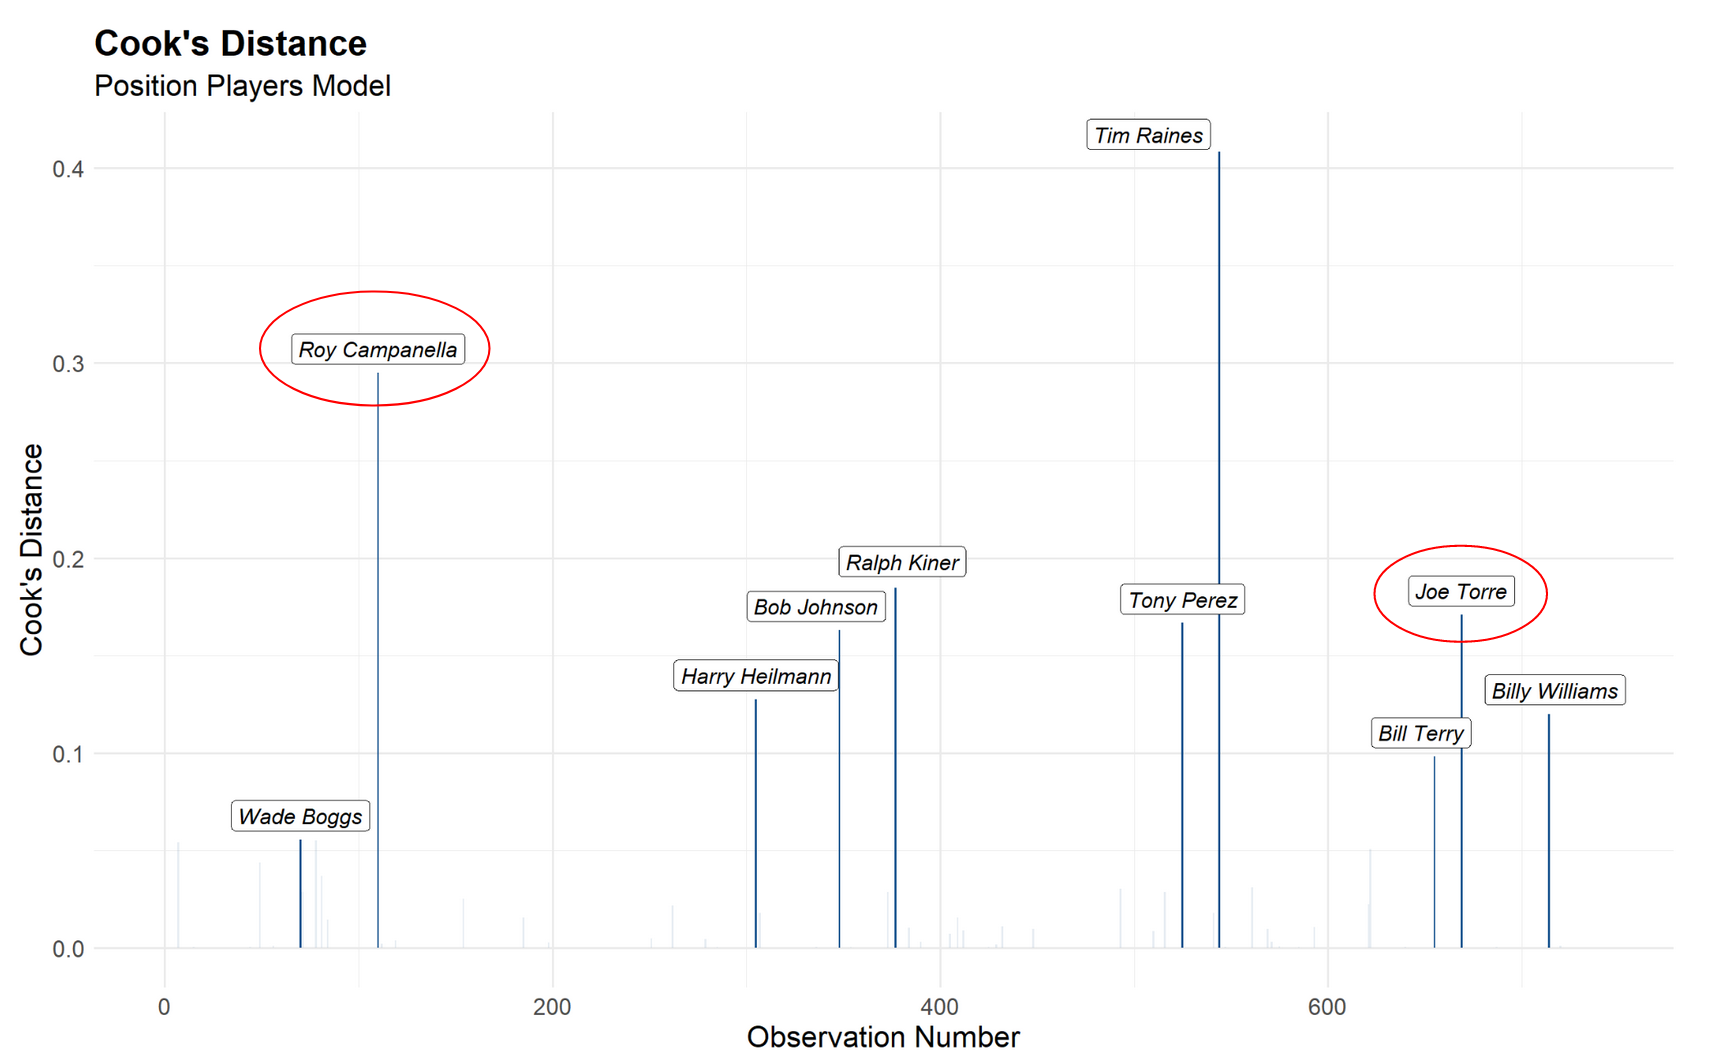
\includegraphics[width=0.49\linewidth,height=0.2\textheight]{../Plots/pos_cooks} 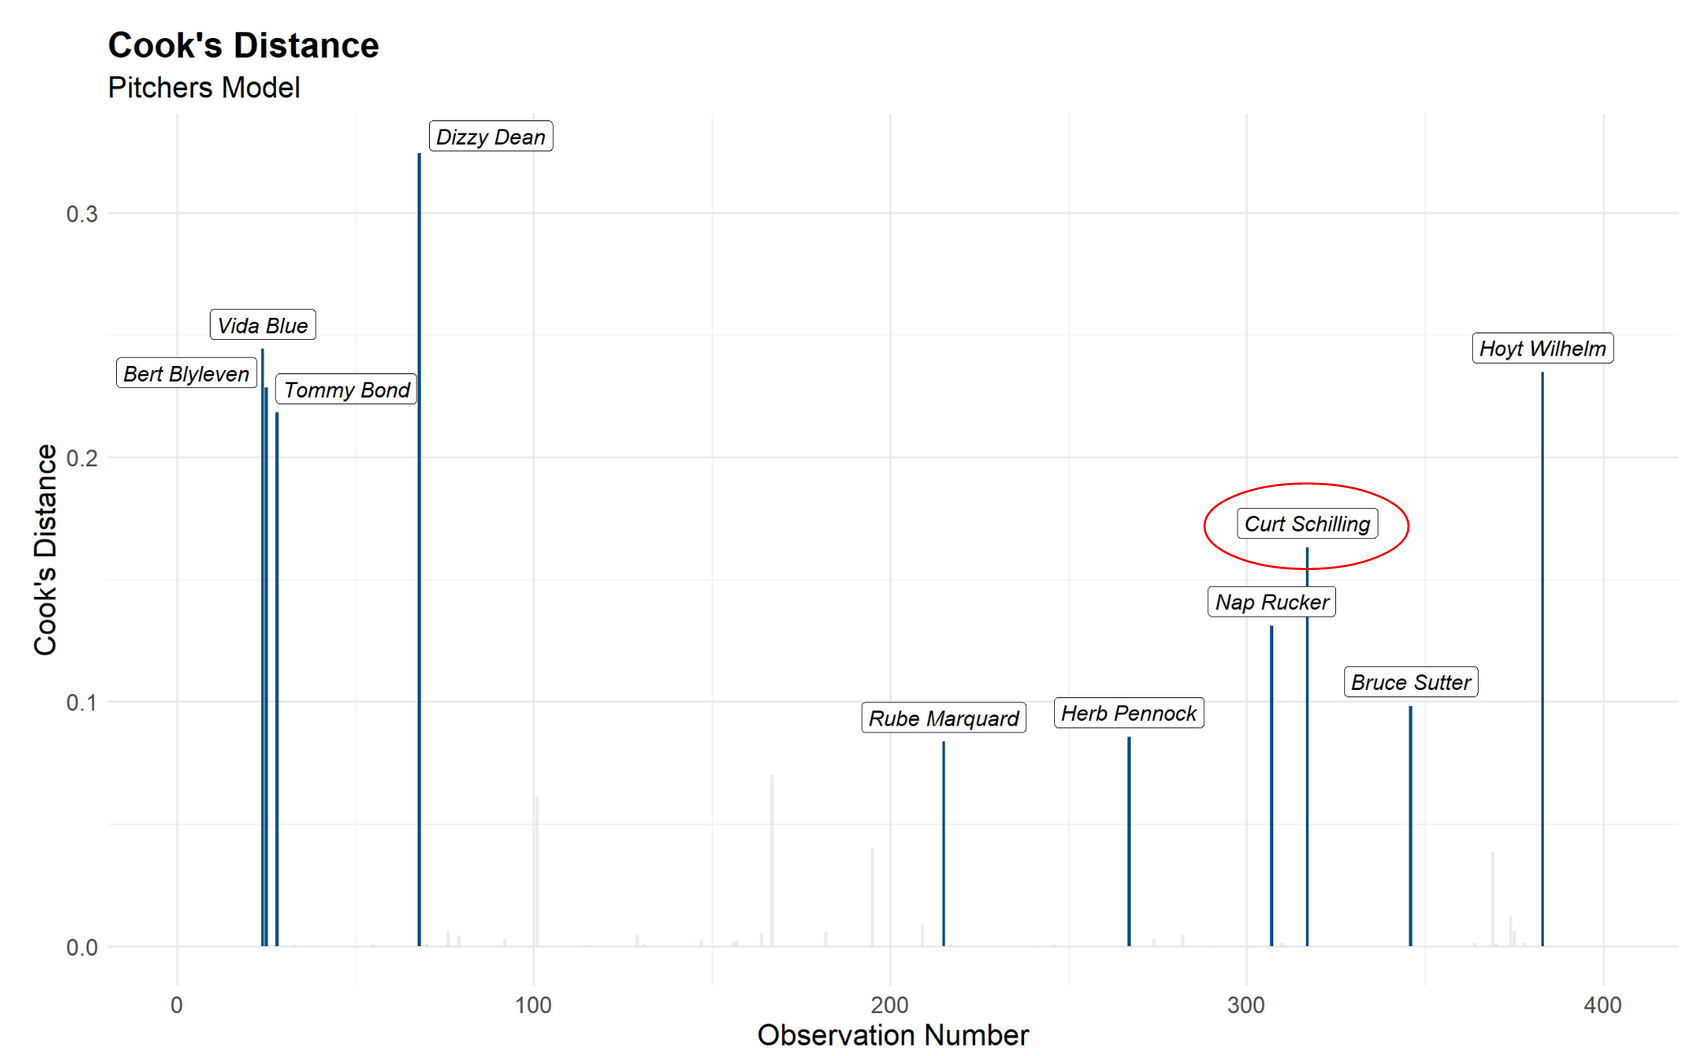
\includegraphics[width=0.49\linewidth,height=0.2\textheight]{../Plots/pitch_cooks} 

}

\caption{Cook's Distance Plots}\label{fig:unnamed-chunk-10}
\end{figure}

These Cook's Distance plots pass the eye test for weird observations.
Joe Torre was inducted more for his contributions to the game as
baseball's Commissioner, and not so much for his prowess as a player.
Roy Campanella's Kansas City Monarch data is not included in his MLB
counting stats, so our model is a bit confused to why he is inducted
even though it's entirely deserving. Curt Schilling's character off the
field has been widely attributed to why he is not elected despite his
successful career.

\hypertarget{trainingtest-set}{%
\subsection{Training/Test Set}\label{trainingtest-set}}

\begin{figure}

\includegraphics[width=0.4\linewidth,height=0.4\textheight]{Report_files/figure-latex/unnamed-chunk-11-1} \includegraphics[width=0.4\linewidth,height=0.4\textheight]{Report_files/figure-latex/unnamed-chunk-11-2} \hfill{}

\caption{K-fold Confusion Matrices}\label{fig:unnamed-chunk-11}
\end{figure}

We can tell above that neither model particularly performed very well on
the test set. While the overall accuracy is high, both models clearly
struggle with correctly identifying a hall of fame player. The
precision, which is the number of true positives out of total positives,
is below 50\% for both models. The same is true for the recall, which is
the number of true positives out of total hall of fame players in the
test set.

\hypertarget{prediction}{%
\subsection{Prediction}\label{prediction}}

In addition to how our model performed on the training data, we wanted
to see how it would work on future prospective hall of fame inductees.
As such, our final prediction results are published on the web
application here:
\textbf{\url{https://klobby19.shinyapps.io/explorable/}}

In terms of our our predictions, we would say that they are, for the
most part, accurate. However, there are a few players in which we
disagree with the model's choice in the position player side, namely
Adrian Beltre and Yadier Molina, both of whom have a low predicted
chance of getting in. This may be because of overfitting to our training
data or it also could be a result of a changing criteria when it comes
to what makes a player hall of fame worthy.

It is also important to note that these predictions are ``now-casting''
not forecasting, since we are essentially assuming that all the players
that we are predicting are all retired. As such, since our model looks
at many counting stats, players who are not retired yet and have low
probabilities to get into the hall of fame can, in theory, improve their
chances by picking up more stats over the rest of their careers.
However, we still believe that our model brings valuable information
regarding players who have retired or are at the end of their careers,
since they are not likely to improve their chances much, if at all.

\hypertarget{discussions-and-conclusions}{%
\section{Discussions and
Conclusions}\label{discussions-and-conclusions}}

\hypertarget{interpretation}{%
\subsection{Interpretation}\label{interpretation}}

The goal of our research question has always been prediction, and thus,
the AIC value which we used to assess our model has left us with many
more parameters than if we used the BIC. Below are selected coefficients
from our final position player and pitching glm objects. We will
interpret them based on the fact that they met our family wise
significance level, and not necessarily because they have a sign or
magnitude which makes sense contextually.

\begin{itemize}
\item
  From the exponentiated \texttt{all\_star} parameter
  \(e^{\beta_{allstar}} = e^{1.321} = 3.75\), we can say for every
  all-star selection of a position player, the odds of being elected
  into the Baseball Hall of Fame increase by 3.75 times when holding all
  other predictors constant. From the 95\% C.I. {[}1.95, 9.38{]}, we are
  95\% confident that for every all-star appearance, the odds of being
  elected into the Hall of Fame increases by 1.95 to 9.38 times. This
  makes sense intuitively, as consistent all-star selections is
  synonymous with consistent player performance. The positive feedback
  loop of baseball writers awards players accolades and then using those
  accolades to justify Hall of Fame election is shown through many
  parameters in both the batter and pitcher models.
\item
  From the exponentiated \texttt{votedByVeterans} parameter
  \(e^{\beta_{votedByVeterans}} = e^{12.89} = 396329\), we can say the
  odds of a pitcher being elected into the Baseball Hall of Fame
  increase by 396329 times if done by the Veterans Committee when
  holding all other predictors constant. From the 95\% C.I. {[}1062,
  39143030000{]}, we are 95\% confident that for every all-star
  appearance, the odds of being elected into the Hall of Fame increases
  by 1062 to 39143030000 times. This seems like an insane result, but
  when you consider how few players are considered by the Veterans
  Committee and how they are almost always elected into the Hall of Fame
  from their consideration, then it makes sense why our number seems so
  ludacris based on our lack of statistical power.
\end{itemize}

We had several fringe parameters for our position player and pitcher
models which did not quite meet our Bonferroni correction significance
levels, but were close. We listed them below on a selection criteria of
being close to significant and interesting. They follow the same
interpretation logic as above.

\begin{itemize}
\tightlist
\item
  Position Players

  \begin{itemize}
  \tightlist
  \item
    Pos2B, 530855280 w/ 95\% C.I. {[}6199, \(2.13 \times 10^{16}\){]}
  \item
    VotedbyVeterans, \(1.46 \times 10^{10}\) w/95\%
    C.I.{[}\(3.69 \times 10^{5}\), \(8.47 \times 10^{19}\){]}
  \end{itemize}
\item
  Pitchers

  \begin{itemize}
  \tightlist
  \item
    Wins, 1.183 w/ 95\% C.I. {[}1.081, 1.388{]}
  \item
    all\_star, 3.286 w/ 95\% C.I. {[}1.72, 10.63{]}
  \end{itemize}
\end{itemize}

\hypertarget{limitations}{%
\subsection{Limitations}\label{limitations}}

We acknowledge some limitations of our processes. Firstly, our binomial
random variable response of being elected into the Baseball Hall of Fame
(\texttt{wein}) has a naturally low probability of success. Therefore,
many cross-validation methods of model selection and assessment may be
problematic in their accuracy and precision. Also, we admittingly have
multicollinearity issues in our model selection, that with additional
time we would like to correct if we can. Additionally, our research
question surrounding Hall of Fame voting is not a perfect science by any
means. Any election process harbors some roots in favoritism,
superficial perception, and dynamic measures of success Baseball Hall of
Fame voting is no different. Lastly, the poor record keeping of baseball
statistics prior to the mid 20th century has imparted many \texttt{NA}s
in our data frames. This greatly reduces the power in which we can
effectively measure which covariates are associated with Hall of Fame
election.

\hypertarget{future}{%
\subsection{Future}\label{future}}

In future research, we would like to solve our issues of inappropriate
predictors and the lack of power they cause. It would interesting to use
time series analysis with election into the Hall of Fame as the
terminating event, while also making use of cohort-predictor-time
variables. It would be interesting to see if we can somehow quantify
popularity of players by possibly looking at their social media pages
(though it might be hard to gauge popularity before the social media
age).

\hypertarget{references}{%
\section{References}\label{references}}

\begin{itemize}
\tightlist
\item
  Fangraphs. (n.d.). Positional Adjustment. Retrieved from
  \url{https://library.fangraphs.com/misc/war/positional-adjustment/}
\item
  Baseball Reference. (n.d.). Baseball Statistics and History. Retrieved
  from \url{https://www.baseball-reference.com/}
\item
  Lahman, S. (n.d.). The Baseball Archive. Retrieved from
  \url{https://www.seanlahman.com/baseball-archive/statistics/}
\item
  Wikipedia. (2021, December 14). List of Major League Baseball players
  suspended for performance-enhancing drugs. In Wikipedia. Retrieved
  from
  \url{https://en.wikipedia.org/wiki/List_of_Major_League_Baseball_players_suspended_for_performance-enhancing_drugs}
\item
  ESPN. (2009, July 31). A-Rod admits using PEDs from 2001-03. Retrieved
  from \url{https://www.espn.com/mlb/news/story?id=4366683}
\item
  RStudio Team (2022). RStudio: Integrated Development for R. RStudio,
  PBC, Boston, MA URL \url{http://www.rstudio.com/}.
\item
  R Core Team (2022). R: A language and environment for statistical
  computing. R Foundation for Statistical Computing, Vienna, Austria.
  URL \url{https://www.R-project.org/}.
\end{itemize}

\hypertarget{appendix}{%
\section{Appendix}\label{appendix}}

\begin{itemize}
\tightlist
\item
  All: General data tidying including the joining, mutation, and
  filtering necessary for analysis. Developed presentation slides and
  report. Quality control of final report.
\item
  Andy: Generated prediction data set for post-testing involving current
  and past players eligible for hall of fame, applied to predictive
  model.\\
\item
  Dante: Proposed research question and gathered initial data sets.
  Delegated tasks based on project needs. Assumptions and issues. Awards
  EDA, Odd ratios interpretation, Cook's Distances, impact of our
  results.
\item
  Kai:
\item
  Kobe: Carried out necessary data scraping tasks for extra variables,
  data visualizations of different concepts, and the shiny app.
\end{itemize}

\end{document}
